\documentclass[11pt, oneside]{article} 
\usepackage{geometry}
\geometry{letterpaper} 
\usepackage{graphicx}
	
\usepackage{amssymb}
\usepackage{amsmath}
\usepackage{parskip}
\usepackage{color}
\usepackage{hyperref}

\graphicspath{{/Users/telliott_admin/Dropbox/Tex/png/}}
% \begin{center} 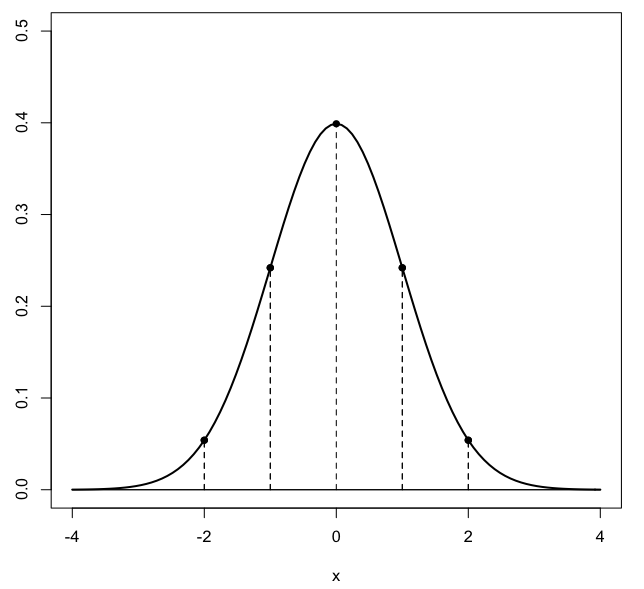
\includegraphics [scale=0.4] {gauss3.png} \end{center}

\title{Examples for limits}
\date{}

\begin{document}
\maketitle
\Large
The limit of a function $f(x)$ at a point $a$ is written
\[ \lim_{x \rightarrow a} f(x) = L \]

The formal definition is:
\[  \forall \ \epsilon > 0, \exists \ \delta > 0 \ | \ \forall \ x, \]
\[ 0 < | x - a| < \delta \Rightarrow | f(x) - L | < \epsilon \]

You tell me the $\epsilon$ you require with $| f(x) - L | < \epsilon$, and I will try to find the right $\delta$.

For a typical function, it's a good guess that $L = f(a)$.
\[ | f(x) - f(a) | < \epsilon \]
which we can write without the absolute value bars (see Triangle write-up):
\[ -\epsilon <  f(x) - f(a) < \epsilon \]

\subsection*{example 1}
Suppose $f(x) = 3x$ and we're interested in the point $a = 5$.  Then set $L = f(a) = 15$.
\[ -\epsilon <  f(x) - f(a) < \epsilon \]
\[ -\epsilon <  3x - 15 < \epsilon \]
\[ - \frac{\epsilon}{3} <  x - 5 < \frac{\epsilon}{3} \]
If we set $\delta = \epsilon/3$ we'll be good.  And in general for a function $f(x) = cx$ with $c$ a constant, at the point $a$, we can use
\[ | x | - a <  \frac{\epsilon}{c} \]

\subsection*{example 2}
Suppose $f(x) = x^2$ and we're interested in the point $a = 2$.  Then set $L = f(a) = a^2 = 4$.
\[ -\epsilon <  f(x) - f(a) < \epsilon \]
\[ -\epsilon <  x^2 - a^2 < \epsilon \]
Now we argue as follows:
\[ x^2 - a^2 = (x - a)(x + a) = |x-a| \ |x + a| \]
and to get started suppose we require that \emph{at least}
\[ | x - a | < 1 \]
\[ -1 < x - a < 1 \]
\[ a - 1 < x < a + 1 \]
\[ 2a - 1 < x + a < 2a + 1 \]
\[ |x + a| < 2a + 1 \]
Then going back to 
\[ |x-a| \ |x + a| < \epsilon \]
\[ |x-a| \ |x + a| < |x - a| \ (2a + 1) < \epsilon \]
and
\[ |x - a| < \frac{\epsilon}{(2a + 1)} \]
Remembering the first condition we set:
\[ |x - a| < \min ( \frac{\epsilon}{(2a + 1)}, 1) = \delta \]
And what we notice is that for $f(x) = x^2$, at least for some $a$ (and depending on the value of $\epsilon$ that is chosen), the value of $\delta$ required depends on $a$.

That should not be too surprising.
\begin{center} 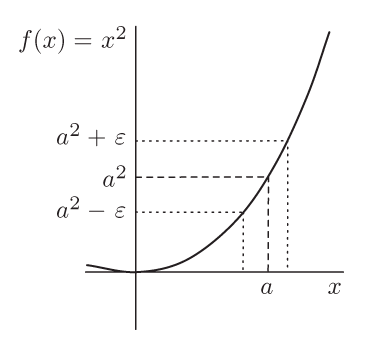
\includegraphics [scale=0.6] {limits2.png} \end{center}
The same $\epsilon$ will require a smaller $\delta$ the farther out we go on the curve.

\subsection*{example 3}
Now consider the inverse function $f(x) = 1/x$.  Suppose we're interested in the point $a = 3$ where we expect the limit to be $L = 1/3$.  For this to be true we must guarantee that
\[ | \frac{1}{x} - \frac{1}{3} | < \epsilon \]
for arbitrary $\epsilon$.

Factor
\[ | \frac{1}{x} - \frac{1}{3} | = | \frac{3 - x}{3x} | = \frac{1}{3} \ \frac{1}{|x|} \ |3 - x|   \]

We showed in the write-up on the triangle inequality that $|a - x| = |x - a|$ so
\[ =  \frac{1}{3} \ \frac{1}{|x|} \ |x - 3|   \]

Here, we need to make sure that $|x|$ is not too \emph{small}, so $1/|x|$ is not too large.

First require that $|x - 3| < 1$ .  Then
\[ -1 < x - 3 < 1 \]
\[ 2 < x < 4 \]
\[ \frac{1}{4} < \frac{1}{x} < \frac{1}{2} \]
This means that $1/x > 0$ so
\[ \frac{1}{|x|} = \frac{1}{x} < \frac{1}{2} \]

We now have
\[ | \frac{1}{x} - \frac{1}{3} | = \frac{1}{3} \ \frac{1}{|x|} \ |3 - x|   \]
provided $|x - 3| < 1$ and also with this condition $1/|x| < 1/2$ so
\[  | \frac{1}{x} - \frac{1}{3} | < \frac{1}{6} \ |x - 3| \]
Hence if $\delta = |x - 3| < 6 \epsilon$, the above expression is $< \epsilon$ and we're done.  Officially we need:
\[ |x - 3| < \min \ (6 \epsilon, 1) \]


\end{document}}